\documentclass[11pt]{article}

% NOTE: To produce blinded version, replace "0" with "1" below.
\newcommand{\blind}{1}


% DON'T change margins - should be 1 inch all around.
\addtolength{\oddsidemargin}{-.5in}%
\addtolength{\evensidemargin}{-.5in}%
\addtolength{\textwidth}{1in}%
\addtolength{\textheight}{-.3in}%
\addtolength{\topmargin}{-.8in}%


\usepackage[utf8]{inputenc}
\usepackage{lipsum}

\usepackage{amsmath,amssymb}
\usepackage{natbib}


\usepackage{amssymb,amsbsy,amsfonts,amsmath,xspace,amsthm}
\usepackage{mathrsfs}
\usepackage{graphicx}


\usepackage{caption}
\usepackage{setspace}
\usepackage{comment}
\doublespacing
\usepackage[margin=1in]{geometry}
\usepackage{enumitem}
\captionsetup[table]{font={stretch=1}}     %% change 1.2 as you like
\captionsetup[figure]{font={stretch=1}}  
\captionsetup[table]{font=small}
\captionsetup[figure]{font=small}
\usepackage{subcaption}
%\usepackage{graphics}
%\usepackage{Sweave}
%\usepackage{JLMR_micro}
\usepackage{multirow}
\usepackage{epstopdf}
\usepackage{epsfig}
%\usepackage{hyperref}
\usepackage[colorlinks,citecolor=blue]{hyperref}

\usepackage{url}
\usepackage[toc,page]{appendix}
\usepackage{float}
\usepackage{natbib}
%\usepackage{enumerate}
\usepackage{color}
\usepackage[dvipsnames]{xcolor}
\usepackage{verbatim}
\usepackage{authblk}
\usepackage[normalem]{ulem}



%\def\proclaim#1{\par \bigskip\noindent {\bf #1}\bgroup\it\ }
%\def\endproclaim{\egroup\par\bigskip}
%\def\proof{\par\noindent{\bf Proof.} \;}
\def\ack{\section*{Acknowledgements}%
  \addtocontents{toc}{\protect\vspace{6pt}}%
  \addcontentsline{toc}{section}{Acknowledgements}%
}


\usepackage{hyperref}
\hypersetup{
    colorlinks=true,
    linkcolor=blue,
    filecolor=magenta,      
    urlcolor=cyan,
    citecolor=blue
}
 
 


\usepackage{amsmath}
\usepackage{graphicx}
\newcommand*{\KeepStyleUnderBrace}[1]{%f
\mathop{%
\mathchoice
{\underbrace{\displaystyle#1}}%
{\underbrace{\textstyle#1}}%
{\underbrace{\scriptstyle#1}}%
{\underbrace{\scriptscriptstyle#1}}%
}\limits
}
\usepackage{mathtools}
\mathtoolsset{showonlyrefs}
\usepackage{amsmath,amssymb,amsthm,bm,hyperref}
\usepackage{dsfont,listings}

 

\usepackage[ruled,vlined]{algorithm2e}
\SetAlFnt{\small}
\SetAlCapFnt{\small}
\SetAlCapNameFnt{\small}

\usepackage{enumitem}
\theoremstyle{definition}
\newtheorem{schm}{Scheme}
\newtheorem*{schm*}{Scheme}
\newtheorem{thm}{Theorem}[section]
\newtheorem{lem}{Lemma}
\newtheorem{prop}{Proposition}
\newtheorem{property}{Property}
\newtheorem{assumption}{Assumption}

\newtheorem{corollary}{Corollary}[section]
\newtheorem{defn}{Definition}
\newtheorem{example}{Example}
\newtheorem{rmk}{Remark}
\newtheorem{clm}{Claim}

\usepackage{xcolor}
\allowdisplaybreaks
\input macros.tex

\setcounter{secnumdepth}{3}
%\bibliographystyle{natbib}

\def\spacingset#1{\renewcommand{\baselinestretch}%
{#1}\small\normalsize} \spacingset{1}
\def\fixme#1#2{\textbf{\color{red}[FIXME (#1): #2]}}
\def\mycomment#1{\textbf{\color{blue}#1}}
\def\ccomment#1{\textbf{\color{ForestGreen}#1}}
\usepackage{hyperref}
\usepackage[parfill]{parskip}
\usepackage{bm}


\newcommand{\Hnorm}[1]{\left\lVert#1\right\rVert_{\tH_\alpha}}
\newcommand{\nullnorm}[1]{\left\lVert#1\right\rVert}
\def\trueB{\mB^{\text{true}}}
\def\newX{\mX_{\textup{new}}}
\def\newy{y_{\textup{new}}}
\def\sign{\textup{sign}}
\def\bayesf{f_{\textup{bayes}}}
\def\bayesS{S_{\textup{bayes}}}
\def\bayespif{f_{\textup{bayes},\pi}}
\def\CNN{\text{\bf \small CNN }}
\def\Lasso{\text{\bf \small Lasso }}
\def\NonparaM{\text{\bf \small NonparaM }}
\def\LogisticM{\text{\bf \small LogisticM }}
 
 
\usepackage{setspace}
\doublespacing
 
\begin{document}

\if1\blind
{   \date{}
  \title{\vspace*{-2cm}\bf Nonparametric learning with matrix-valued predictors in high dimensions}
\author{\vspace*{-.3cm} Chanwoo Lee$^{1}$, Lexin Li$^2$, Hao Helen Zhang$^3$, and Miaoyan Wang$^1$\\\vspace*{-.2cm}
$^1$Department of Statistics, University of Wisconsin-Madison\\
$^2$Department of Biostatistics and Epidemiology, University of California at Berkeley\\
$^3$Department of Mathematics, University of Arizona\\
}

    \maketitle
} \fi

\if0\blind
{
 \date{}
  \title{\vspace*{-2cm}\bf Nonparametric learning with matrix-valued predictors in high dimensions}
\author{}
\maketitle
} \fi




\vspace{-.5cm}
\begin{abstract}
We consider the problem of learning the relationship between a binary label response and a high-dimensional matrix-valued predictor. Such data problems are important in brain imaging studies, sensor network localization, and personalized medicine. Existing supervised analysis typically takes a parametric procedure by imposing a pre-specified relationship between variables. Parametric methods, however, often perform poorly under misspecified models, especially in the high dimension, low sample size settings. Here, we develop a learning reduction framework to address a range of learning tasks from classification to regression that account for matrix-valued predictors. The proposal achieves interpretable prediction using a low-rank two-way sparse representation of the target function. Unlike earlier approaches, our regression model is distribution-free and adapts to the possibly non-smooth, non-linear function of interest. Estimation consistency, and convergence rate are established. We demonstrate the advantage of our method over previous approaches through numerical analyses and applications. 
\end{abstract}
\vspace{-.2cm}
\noindent%
{\it Keywords:}  Nonparametric learning, high-dimensional matrix-valued predictors, sparse and low-rank models, classification, regression, feature selection

\vspace{-.5cm}
\section{Introduction }
\vspace{-.3cm}
Consider a statistical learning setting where we would like to model the relationship between a matrix-valued predictor $\mX \in \mathbb{R}^{d\times d}$ and a binary label response $Y\in\{-1,1\}$. Matrix-valued predictors ubiquitously arise in modern applications. One example is from electroencephalography studies of alcoholism. The data set records voltage value measured from 64 channels of electrodes on 256 subjects for 256 time points~\citep{zhou2014regularized}. Each feature is a $256\times 64$ matrix and the response is a binary indicator of subject being alcoholic or control. Another example is pedestrian detection from image data. Each image is divided into 9 regions where local orientation statistics are generated with a total of 22 numbers per region. This yields a $22 \times 9$ matrix feature and a binary label response indicating whether the image is pedestrian~\citep{Shashua2004Pedestrian}.  Our motivating problem  comes from brain network analysis. In this study, each individual in the sample is represented by their own brain network, and the nodes (brain regions of interest) shared across all networks are mapped onto a common atlas. Human connectom project~\citep{wang2017bayesian} has 68 brain nodes extracted from six functional brain regions. A connectivity is computed for every pair of nodes, resulting in an adjacency matrix of size 68 $\times$ 68 for each individual. This brain connectivity network is used to predict the individual's disease probability. 

% Two main approaches have been used in the existing literature. One approach is to reduce the network to its global summary measures such as the average degree, clustering coefficient, or average path length, and use those measures as features for disease predicting. However, this approach cannot get the most out of the original dataset because summary measures results in information loss.  An alternative approach is to treat connectivity network as a ``bag of non-ordered edges,'' which essentially vectorized the adjacency matrix. This approach ignores the network nature of the predictor and suffers from high dimensionality.


The key challenge with matrix-valued predictors is the high-dimensional, complex structure in the feature space. One approach is to transform the feature matrices to vectors and apply classical methods such as Lasso \citep{friedman2010regularization}. However, this vectorization would destroy the structural information of the data matrices. 
Matrix-valued predictors represent various aspects of data features, including global structure (e.g.\ clustering patterns, community hubs) and local structure (e.g.\ node degrees, edge connections).
The vectorization cannot consider those aspects.
Traditionally, many learning problems are addressed through distribution assumption such as logistic regression, linear discriminant analysis (LDA) \citep{agresti1998approximate}, and group lasso \citep{relion2019network}. In many applications, however, it is often difficult to  justify the assumptions. Groupo lasso is only designated for network data and the model assumptions made on logistic regression or LDA become challenging for matrix features because of high dimensionality.
For those reasons, nonparametric approaches such as k-nearest neighbors, decision trees, and convolutional neural network (CNN) \citep{chollet2015keras} have been popular in prediction problem.
In the above examples and many other studies, however, researchers are interested in {\it interpretable prediction}, where the goal is to not only make accurate prediction but also identify features that are informative to the prediction. The current nonparametric methods lack interpretability that can help researchers to find out new scientific facts. 

We propose new learning framework that respects the matrix structure of the predictors and produces interpretable results without distribution assumption. We consider three main learning problems: classification, level set estimation, and regression in a relation to the above examples.
We utilize a low-rank two-way sparse matrix representation of the targeted regression function. The representation enables efficient variable selection in the high-dimensional matrix learning. We achieve theoretical guarantees for classification errors and derive rates of convergence of the proposed regression in L1 sense. 
Our numerical analyses suggest that the proposed method is highly competitive and applicable.

% The classification problem has long been interested. Many attempts have been developed and performed well for example, decision tree, nearest neighbor, neural network and support vector machine to name a few. However, most of methods have focused on vector valued features. In many classification problems, the input features are naturally represented as matrices or tensors rather than vectors. 


% Knowledge about the class probability itself is of significant interest and can tell us the confidence of the outcome of classification. Traditionally, the regression problem is addressed through distribution assumption like logistic regression or linear discriminant analysis (LDA). In many applications, however, it is often difficult to  justify the assumptions made in logistic regression or satisfy the Gaussian assumption in LDA. These issues become more challenging for matrix features because of high dimensionality.
% We establish distribution free method for estimating the regression function based on level set estimation. 

% Other examples can be found in medical decision making. In Osteosarcoma treatment, the degree of tumor necrosis is used to guide the choice of postoperative chemotherapy \citep{man2005expression}. Patients with $\geq 90 \%$ necrosis is labeled as 1, which is response variable $y$. Suppose that $\mX$ is a feature matrix collected from the patient such as gene expression levels on each tissue. Knowledge of the regression level set is needed to allow effective postoperative chemotherapy without a biopsy. 
% We consider a nonparametric way to estimate the $\pi$-level set of the regression function based on classification problem.

%  {\color{red}(three sources of error)}. Mention in abstract or introduction. 
 
{\bf Notation:} Let $f$ be a function from $\tX$ to $\mathbb{R}$. We denote $\sign f$ as the sign function such that $\sign f(\mX)=1$ if $f(\mX)>0$ and $\sign f(\mX)=-1$ if $f(\mX)\leq 0$, for all $\mX\in \tX$.  Let $\mathds{1}(\cdot)$ denote the indicator function. A set $A$ uniquely determines an indicator function $\mathds{1}(\mX\in A)$. We use the shorthand $\sign (\mX\in A)\stackrel{\text{def}}{=}2\mathds{1}(\mX\in A)-1$ to denote the sign function induced by the set $A$.  Given a $d_1$-by-$d_2$ matrix $\mB$, we use $\mB_i$ to denote the $i$-th row of $\mB$, where $i\in[d_1]$. We use $\newnormSize{}{\cdot}_p$ to denote the $p$-norm for vectors for $p\geq 0$. The $(p,q)$-norm of a matrix $\mB$ is defined as $\newnormSize{}{\mB}_{p,q}=\newnormSize{}{\mb}_q$, where $\mb=(\newnormSize{}{\mB_1}_p,\ldots,\newnormSize{}{\mB_{d_1}}_p)\in\mathbb{R}^{d_1}$ consists of the $p$-norms for each of the rows in $\mB$. In particular, $\newnormSize{}{\mB}_{1,0}=\#\{i\in [d_1]\colon \mB_i\neq 0\}$ denotes the number of non-zero rows in $\mB$.
We denote $a_n\asymp b_n$ if $\lim_n b_n/a_n\rightarrow c$ for some constant $c>$ and denote $a_n\lesssim b_n$ if $\lim_n b_n/a_n\rightarrow 0.$
 
\vspace{-.5cm}
\section{Three learning problems}
\vspace{-.3cm}
In this section we present the main learning goals of our interest. Let $\mX\in\mathbb{R}^{d_1\times d_2}$ denote the matrix-valued predictor, $y\in\{-1,1\}$ denote the binary label response, and $\mathbb{P}_{\mX,Y}$ denote the unknown joint probability distribution over the pair $(\mX,y)$. Suppose that we observe a sample of $n$ training data points, $(\mX_1,y_1),\ldots,(\mX_n,y_n)$, identically and independently distributed (i.i.d.) according to $\mathbb{P}_{\mX,y}$. Let $(\mX_{\text{new}},y_{\text{new}})$ be a new test point drawn independently from the same distribution. Our goal is to predict $y_{\text{new}}$ given the new feature value $\mX_{\text{new}}$. When no confusion arises, we often omit the subscript ``new'' and simply write $(\mX,y)$ for the prototypical test point. Note that  $y$ is a Bernoulli random variable with conditional probability $p(\mX)\stackrel{\text{def}}{=}\mathbb{P}(y=1|\mX)$, and we generally make no parametric assumptions on the marginal distribution $\mathbb{P}_{\mX}$ or form of $p(\mX)$. 

%The problem of learning is to find a decision function $f\colon \mathbb{R}^{d_1\times d_2}\to \mathbb{R}$ that minimizes certain expected risk $R(f)$ under the unknown distribution $\mathbb{P}_{\mX,y}$. The expected risk $R(f)$ is a functional over a given class of candidate functions $f\in\tF$; the form of risk depends on the specific learning goals which are detailed in the next paragraph. 

We consider three learning problems: classification, level set estimation, and regression. 

\begin{enumerate}[label={2.\arabic*},wide, labelwidth=!, labelindent=0pt]
\item {\it Classification}: Classification is the problem of predicting the label $y\in \{-1,1\}$ to which a new observation $\mX$ belongs. A prediction rule (also called a classifier) decides that $y=1$ if $\mX\in S$ and $y=0$ if $\mX \not\in S$, where $S$ is a Borel subset of $\mathbb{R}^{d_1\times d_2}$. Because a set $S$ uniquely defines an $\{-1,1\}$-valued sign function in the predictor space, we will use the term ``classifier'' to denote both the set $S$ and its associated sign function. We formulate the classification problem as choosing a classifier $S\in \tS$, from a given set of candidate classifiers $\tS$, that minimizes the expected classification error, 
\begin{equation}\label{eq:classloss}
R(S)=\mathbb{P}\left[y\neq \sign(\mX\in S)\right].
\end{equation}
 The expected classification error $R(S)$ is also referred to as the classification risk. When the candidate set $\tS$ consists of all Borel subsets of $\mathbb{R}^{d_1\times d_2}$, the minimizer of~\eqref{eq:classloss} is called the Bayes classifier.
In practice the population joint distribution $\mathbb{P}_{\mX,y}$ is unknown, so the objective function~\eqref{eq:classloss} and the minimizer  need to be estimated through the data. Our first goal is to estimate the Bayes classifier for matrix classification:

{\bf Question 1.} When matrix dimension $d_1d_2$ far exceeds the sample size $n$, how to efficiently perform matrix classification without much assumption on $\mathbb{P}_{\mX,y}$?



\item {\it Level set estimation}: The problem of level set estimation generalizes the classification task. 
%Let $p(\mX)=\mathbb{P}(y=1|\mX)$ denote the conditional probability function over the matrix space $\mathbb{R}^{d_1\times d_2}$. 
%Note that $p(\mX)$ is a bounded function over $\mathbb{R}^{d_1\times d_2}$, because of $y$ is labeled by $\pm 1$. 
For a given $\pi\in(0, 1)$, the $\pi$-level set of the conditional probability function $p(\mX)$ is defined as
\begin{equation}\label{eq:level}
\bayesS(\pi) = \{\mX\in\mathbb{R}^{d_1\times d_2}\colon p(\mX)\geq \pi\}.
\end{equation}
%The set $S(\pi)$ uniquely defines an indicator function, $\mathds{1}\{\mX\in S(\pi)\}$, over the matrix space. 
It is known that  the set $\bayesS(\pi)$ optimizes the weighted classifier risk~\citep{willett2007minimax,scott2007regression,wang2008probability}. Specifically, among all Borel subsets of $\mathbb{R}^{d_1\times d_2}$, the set $S_{\text{bayes}}(\pi)$ is the global minimizer of the expected $\pi$-weighted classification error,
\begin{equation}\label{eq:risklevel}
%R(f)=\mathbb{E}_{\mX,y}\left[w(y)I\left(y\neq \sign f(\mX)\right) \right],
R_\pi(S)=\mathbb{E}\left[ w_{\pi}(y)\mathds{1}(y\neq \sign(\mX\in S))\right],
\end{equation}
where we define $w_{\pi}(y)=1-\pi$ or $\pi$ depending on $y=1$ or $-1$. In light of~\eqref{eq:classloss} and~\eqref{eq:risklevel}, the level set problem is an extension of the usual classification from equal weight $\pi=1/2$ to general weight $\pi \in(0,1)$. Accurate level set estimation plays an important role in applications of geographical elevation maps, imaging contour detection, and motion tracking. We consider the following question:

{\bf Question 2.} How to simultaneously estimate the level set and identify important variables in the matrix-valued predictors $\mX$, for the goal of interpretable prediction?


\item {\it Nonparametric regression}: The problem of nonparametric regression is to estimate the conditional mean $\mathbb{E}(y|\mX)$ as a multivariable function in the predictor space. In the our contexts, the nonparametric regression is equivalent to the estimation problem of conditional probability $p(\mX)=\mathbb{P}(y=1|\mX)=\frac{1}{2}(\mathbb{E}(y|\mX)+1)$. Throughout the paper we will focus on $p(\mX)$ and refer to it as the regression function. Our final goal is the function estimation:

{\bf Question 3.} How to learn the regression function $p(\mX)$ in the high-dimensional matrix space?
\end{enumerate}


% Matrix-valued predictors impose unique challenges to the aforementioned three problems. We consider nonparametric learning without imposing particular function forms of $p(\mX)$, and we allow matrix dimension $d_1d_2$ to grow sub-exponentially with the sample size $n$. This scenario is important yet notably hard for several reasons. First, nonparametric methods typically rely on some notion of local smoothness to learn function forms. Efficient extraction of neighborhood structure in the matrix space has yet to explore. Second, matrix-valued predictors often lead to high dimension problem in which feature dimension diverges with the sample size. Accurate prediction is statistically difficult in such a setting. Unlike parametric models, non-parametric learning makes little assumption on the variable relationships, which adds further complexity to interpretation. Achieving accurate prediction while maintaining descriptive simplicity will be our goal. 

%“learning reduction” from one supervised learning problem to another which is more fundamental or better understood. Our approach finds classification rule first and address the level set estimation and regression problem in order. We blend the level set approach in functional optimization with label-sensitive classification in statistical machine learning, and take the best out of the two worlds. 

The three problems of our interest represent a range of learning tasks with increasing difficulties. Classification is a special case of level set estimation with $\pi=1/2$, whereas the level set is a discrete approximation of the regression function. A common approach is to address regression first, and then solve the earlier two using plug-in estimates (Figure~\ref{fig:diagram}a). This procedure, however, undermines the fact that regression is generally harder than the other two. Indeed, as we show in Section~\ref{sec:theory}, regression has a slower convergence rate compared to that of classification. 
Ignorance of the increased complexity violates Vapnik’s maxim: \emph{When solving a given problem, one should try to avoid solving a more general problem as an intermediate step.}  We follow Vapnik's principle to develop a ``learning reduction'' approach by relating the regression to classification, the latter of which is more fundamental and easier to address. In the next section, we propose to address classification first and solve the regression based on ``learning reduction'' framework (Figure~\ref{fig:diagram}b).


\begin{figure}\centering
\includegraphics[width=0.9\textwidth]{level.pdf}\hspace{1cm}
\caption{(a) Our learning reduction approach (solid line) to three learning problems and classical plug-in approaches (dashed line). (b) Schematic diagram for nonparametric function estimation via level set estimation. Figure (b) is modified from~\cite{gibou2018review}. }\label{fig:diagram}
\end{figure}

\vspace{-.5cm}
\section{Estimation}\label{sec:idea}
\vspace{-.3cm}%The theoretical and algorithmic benefits of our approach will be demonstrated in Sections~\ref{sec:theory}-\ref{sec:algorithm}.
% \subsection{Classification and level set estimation for high dimensional matrices}
% \vspace{-.2cm}
% We  describe the choice of candidate classifiers $\tS$ in~\eqref{eq:risklevel}. We rewrite the optimization~\eqref{eq:risklevel} as the minimization over continuous-valued functions,
% \begin{equation}\label{eq:optimization}
% \bar S(\pi) = \{\mX\colon\bar f(\mX)\geq 0\},\quad  \text{with}\quad  \bar f(\mX)= \argmin_{f\in\tF}\mathbb{E}\left[w_\pi(y)\mathds{1}(y\neq \sign f(\mX))\right],
% \end{equation}
% where $\bar f\in\tF$ is a continuous-valued function from $\mathbb{R}^{d_1\times d_2}$. The choice of $\tS$ thus reduces to the choice of function family $\tF$. A desirable $\tF$ should balance the prediction and interpretability; i.e., $\tF$ should be flexible enough for accurate prediction while being simple enough for high interpretability. 
Our building block is to use level sets to estimate regression function $p$ through classifications. The level set approach bridges the two sides of a same coin -- characteristic (set indicator) functions in functional analysis and weighted classifications in statistical learning.  Let $\Pi=\{{1\over H},{2\over H} \ldots, {(H-1)\over H} \}$ be a sequence of evenly spaced points in $[0,1]$, where $H\in\mathbb{N}_{+}$ is the resolution parameter. We introduce an $H$-step function from $\mathbb{R}^{d_1\times d_2}$ to $[0,1]$,
\begin{equation}\label{eq:stepfunction}
\hat p(\mX)= {1\over 2H}  \sum_{\pi \in \Pi} \sign (\mX\in \hat S(\pi))+{1\over 2},
\end{equation}
where, for every $\pi\in\Pi$, the set $\hat S(\pi)\subset \mathbb{R}^{d_1\times d_2}$ is estimated classifiers we will obtain from \eqref{eq:large-margin}.
Figure~\ref{fig:method} shows the schematic diagram of our approaches. We use a sequence of weighted classifications to estimate the level sets $\bayesS(\pi)$ in the matrix space, and then approximate the target regression function $p(\mX)$ via the function $\hat p(\mX)$. 


\begin{figure}[http]
\centering
\includegraphics[width=13cm]{demo_method.pdf}
\caption{Matrix nonparametric regression via weighted classification. We use a sequence of $\pi$-weighted classification to find level sets in the matrix space, and then approximate the target regression function.}\label{fig:method}
\end{figure}

For the level set estimation $\hat S(\pi)$,
we consider the weighted matrix classification with general $\pi\in(0,1)$. The usual classification is naturally obtained by setting $\pi=1/2$. We propose to estimate the matrix classifier based on penalized empirical surrogate risk minimization,
\begin{align}\label{eq:large-margin}
\hat S(\pi) = \{\mX \colon \hat f_\pi(\mX) \geq 0\}, \quad \text{where}\quad \hat f_\pi=\min_{f\in\tF}\left\{ {1\over n}\sum_{i=1}^n w_{\pi}(y_i)\ell\left(y_if(\mX_i)\right)+ \lambda \FnormSize{}{f}^2\right\},
\end{align}
where $w_\pi(y) = 1-\pi $ if $y = 1$ and $w_\pi(y)=\pi$ if $y = -1$ is the weight for two labels, $\tF$ is the considered function family, the surrogate loss $\ell(z)\colon \mathbb{R}\mapsto \mathbb{R}_{\geq 0}$ is a non-increasing function of the margin $z=yf(\mX)$,  $\lambda>0$ is the penalty parameter, and we define the penalization term $\FnormSize{}{f}$, according to $\tF$.
Examples of large-margin loss functions are hinge loss $\ell(z) = (1-z)_+$ for support vector machines, logistic loss $\ell(z) =\log(1+e^{-z})$ for important vector machines, and $\psi$-loss $\ell(z)=2\min(1,(1-z)_+)$, where $z_{+}=\max(z,0)$. The properties and choices of surrogate loss have been studied earlier~\citep{scott2011surrogate,bartlett2006convexity}. We choose hinge loss for parsimony; our framework applies equally to other common large-margin losses~\citep{scott2011surrogate}.

The estimation~\eqref{eq:large-margin} generalizes the population formulation~\eqref{eq:risklevel} from three aspects. First, the population expectation in~\eqref{eq:risklevel} is replaced by the empirical sample average, which is common in statistical learning problems with i.i.d.\ assumption. Second, we add the ridge penalization $\lambda\FnormSize{}{f}^2$ to control the magnitude of the classifiers. The oracle tuning parameter $\lambda$ depends on the sample size and the problem dimension.  In practice, we choose $\lambda$ in a data-adaptive fashion via cross validation. Third, we replace the binary loss in~\eqref{eq:risklevel} by a more manageable large-margin loss. This relaxation allows us to leverage efficient large-margin algorithms while maintaining desirable statistical performance under mild assumptions. 


We propose the linear function family $\tF$ with low-rank two-way sparse matrix coefficients,
\begin{align}\label{eq:class}
\tF(r,s_1,s_2)=\{f\colon \mX\mapsto \langle \mX, \mB \rangle +b \ \big|\ \text{rank}(\mB)\leq r, \ \text{supp}(\mB)\leq (s_1,s_2), \ \mB\in\mathbb{R}^{d_1\times d_2},\ b\in\mathbb{R}\},
\end{align}
where $\text{rank}(\mB)$ denotes the rank of the coefficient matrix, and $\text{supp}(\mB)$ denotes the two-way sparsity, with $s_1=\newnormSize{}{\mB}_{1,0}$ and $s_2=\newnormSize{}{\mB^T}_{1,0}$ being the numbers of non-zero rows and columns of $\mB$, respectively. We define penalization term in \eqref{eq:large-margin} as $\FnormSize{}{f} = \FnormSize{}{\mB}$. For the theory, we assume that $(r,s_1,s_2)$ are known; the adaptation to unknown $(r, s_1, s_2)$  is described in Section~\ref{sec:data}. 
The low-rank two-way sparse classifier~\eqref{eq:class} enables efficient variable selection in the high-dimensional matrix learning, thereby achieving interpretability. 

 



\vspace{-.5cm}
\section{Statistical properties}\label{sec:theory}
\vspace{-.3cm}
To address accuracy of weighted classification and regression, we need to control the behavior of the regression function near the level set boundaries $\partial S_{\text{bayes}}(\pi) = \{ p(\mX)= \pi\}$. We call a level $\pi\in[0,1]$ a mass point if the level set boundary $\partial \bayesS(\pi)$ has non-zero measure under $\mathbb{P}_{\mX}$. Let $\tN=\{\pi\in[0,1] \colon \mathbb{P}\left[p(\mX)=\pi\right]\neq 0\}$ denote the collection of mass points in $p(\mX)$.

\begin{defn} [Global regularity]\label{ass:decboundary}
A function $p(\mX)$ is $\alpha$-globally regular, if 
\begin{enumerate}[label=(\roman*)]
\item $p(\mX)$ has finitely many mass points, i.e., $|\tN|\leq C'$ for some constant $C'<\infty$; and 
\item 
there exists a global constant $C>0$ such that, for all $\pi \notin \tN $,
\[
\mathbb{P}(|p(\mX)-\pi|\leq t)\leq Ct^{\alpha/(1-\alpha)}, \quad \text{for }t\in \left(0,\rho(\pi,\tN)\right),
\]
where $\rho(\pi,\tN)\stackrel{\text{def}}{=}\min_{\pi'\in \tN} |\pi-\pi'|$  denotes the distance from $\pi$ to the nearest mass point in $\tN$. When $\tN = \phi$, we define $\rho(\pi,\tN)=1$.
\end{enumerate}
\end{defn}

%\begin{assumption}[Uniform smoothness]\label{ass:decboundary}
%Let $\tN$ denote the collection of levels for which the level set boundary $\partial \bayesS(\pi)$ has non-zero measures under $\mathbb{P}_{\mX}$; that is, $\tN=\left\{\pi\in[0,1]\colon \mathbb{P}_{\mX}[p(\mX)=\pi]\neq 0\right\}$.  The regression function is assumed to satisfy $|\tN|\leq C'<\infty$, meaning $\tN$ has at most finite elements. Furthermore, there exist constants $\alpha\in[0,1]$ and $C>0$, such that
%\[
%\max_{\pi \in \Pi/\tN}\mathbb{P}\left(|p(\mX)-\pi|\leq t \right) \leq Ct^{\alpha \over 1-\alpha},\quad \text{for all }t\in[0,1/H],
%\]
%for all $H\in\mathbb{N}_{+}$. When $\alpha=1$, the right-hand side of the inequality is interpreted as zero.  
%\end{assumption}
Definition~\ref{ass:decboundary} uniformly control the behavior of $p(\mX)$ across possible $\pi$. If Deifinition~\ref{ass:decboundary}(ii) holds for fixed $\pi\in[0,1]$, we call a function $p(\mX)$ $(\pi,\alpha)-$locally regular.
The $\alpha$ quantifies the concentration of probability mass $p(\mX)$ and determine the estimation accuracy. $\tN$ is a collection of the weights whose classification task is difficult because the deviation of $p(\mX)$ from $\pi$ is too small. We make the number of poor weighted classifications  negligible in regression from Definition~\ref{ass:decboundary}(i). 


% It is worth noting that the imposed range $(\alpha,\beta)\in[0,1]^2$ puts no constraint to the target function, and in fact, we show that the admissible pair is always restricted in a triangle region of $[0,1]^2$ (See Figure~\ref{fig:diagram}c). Furthermore, the noise level $(\alpha, \beta)$ in~\eqref{eq:identity} is solely determined by the probabilistic distribution of $p(\mX)$ viewed as a random variable transformed from $\mX$ via the function $p(\cdot)$. The following characterization sheds light on the statistical nature of the identifiability and provides an easier way to assess the noise level. 

% \mycomment{To Chanwoo: please double check the admissible region $(\alpha,\beta)$. Distinguish two cases: admissible $(\alpha,\beta)$ for a single $\pi$, vs. admissible $(\alpha,\beta)$ as the worst case over all possible $\pi \in \Pi$. The latter region should be depicted as the lower envelop of the former, i.e. two points $\{(\alpha_i,\beta_i)\}_{i=1,2}$ in the gray area should imply the intersection point $(\min(\alpha_1,\alpha_2),\min(\beta_1,\beta_2))$ in the gray area.}
% \fixme{Chanwoo}{
% Another expression of \eqref{eq:mass} is 
% \begin{align}
%     \mathbb{P}\left(\left|p(\mX)-\pi \right|\leq {t\over H}\right) \leq C H^{{1-\beta\over 1-\alpha}}\left(t\over H\right)^{\alpha\over 1-\alpha},\quad \text{for all }t\in[0,1] \text{ and all }H\in \mathbb{N}_{+}.
% \end{align}
% We can think of the part $\left(t\over H\right)^{\alpha\over 1-\alpha}$ as best approximation of $p(\mX)$ around $\pi$ and $C H^{{1-\beta\over 1-\alpha}}$ as corresponding coefficient given $H$. By reflecting the above perspective, we have 
% \mycomment{I like the use of $C(H,\alpha)$. Looks much neat!}
% \begin{align}\label{eq:pi}
%     \mathbb{P}\left(\left|p(\mX)-\pi \right|\leq {t\over H}\right) \leq C(H,\alpha)\left(t\over H\right)^{\alpha\over 1-\alpha},\quad \text{for all }t\in[0,1] \text{ and all }H\in \mathbb{N}_{+}.
% \end{align}
% The coefficient $C(H,\alpha)$ reflects that the coefficient can be different according to $\pi$. The way we overcome this possible different coefficients is to find good $\beta$ such hat $C(H,\alpha)\leq CH^{1-\beta\over 1-\alpha}$. 
%  One illustrative example is the case of $p(\mX) = e^{\mX}/(1+e^{\mX})$ where $\mX$ is uniformly distributed. 
% \begin{align}
%     \mathbb{P}\left(\left|p(\mX)-\pi \right|\leq {t\over H}\right) &=\mathbb{P}\left(p^{-1}(\pi-t/H)\leq \mX\leq p^{-1}(\pi+t/H)\right) \\&= p^{-1}(\pi+t/H)-p^{-1}(\pi-t/H)\\&=  (p^{-1})'(\pi^*)\frac{t}{H}\\&= \frac{1}{\pi^*(1-\pi^*)}\frac{t}{H}\\&\leq H\times \frac{t}{H}.
% \end{align}
% The third equality used mean value theorem where $\pi^*\in(\pi-t/H,\pi+t/H)$ and the equality holds because $t/H < 1/H$ (there is no sharp change in the neighborhood). Here we set $\alpha = 1/2$ and  we have $C(H,\alpha) = \frac{1}{\pi^*(1-\pi^*)}$ which can be viewed as a function of $\pi,H,\alpha$. \mycomment{How does this resolve the earlier issue you mentioned? That is, $p(\mX)$ is bounded because $\mX$ is bounded, which in turn suggests no $H$ in the bound of $C(H,\alpha)$.} \ccomment{In the case where $\mX\in[-n,n]$ and $p(a<\mX<b) = (b-a)/2n$, we still have 
% \[ \mathbb{P}\left(\left|p(\mX)-\pi \right|\leq {t\over H}\right) \leq \frac{H}{2n}\times \frac{t}{H}.
% \]
% To have tighter bound we can define
% \[\pi* = \min_{\pi\in\Pi}\{\pi\colon \max_{\mX\in[-n,n]}p(\mX)\leq \pi\}.
% \]
% Then we have 
% \[ \mathbb{P}\left(\left|p(\mX)-\pi \right|\leq {t\over H}\right) \leq \frac{1}{2n\pi^{**}(1-\pi^{**})}\times \frac{t}{H},
% \]
% where $\pi^{**} \in(\max_{\mX\in[-n,n]}p(\mX),\pi^*).$ Then we have $\beta = 1$ and $\alpha = 1/2$.
% In the case where $\mX \sim N(0,1)$, when $\pi = (H-1)/H$ we have
% \begin{align}
%     \mathbb{P}\left(\left|p(\mX)-\pi \right|\leq {t\over H}\right)&\leq \mathbb{P}\left(\log\left({\pi-t/H\over 1-\pi+t/H}\right)\leq p(\mX)\right)\leq e^{-\log\left({\pi-t/H\over 1-\pi+t/H}\right)}\leq t/H.
% \end{align}
% What the above example implies is that there is a case where $\beta$ is not 0 or 1 because we need to uniformly control $C(H,\alpha)$ which varies according to $H$.
% } 
% By setting $\beta = 1/2$ we make the upper bound $C(H,\alpha) < H$. In this sense, I think we can find many combinations of $(\alpha,\beta)$ that can satisfy \eqref{eq:mass}. My current question is what combination is the best \mycomment{ The largest $(\alpha,\beta)$ is the best} or are there any good way to set $\beta$ given $\alpha$ that can guarantee uniqueness? \mycomment{This is exactly the question we should look into. Existence? yes, because every function $p(\mX)$ satisfies $(\alpha,\beta)=(0,0)$ in the worst case. Optimally? not know yet. This reduces to the question ``How to find the largest $\beta$ given $\alpha$''? Current answers: (1) yours $\beta\in\{1-\alpha,1\}$; (2) mine $\beta \in [1-\alpha, \min(2-2\alpha,1)]$.}
% (May be we don't have to have uniqueness, existence of $(\alpha,\beta)$ would be enough for theoretical convergence).}

% \begin{thm}[Equivalent characterization of identifiability]\label{thm:noise}
% The conversion condition~\eqref{eq:identity} is equivalent to
% \begin{equation}\label{eq:mass}
% \max_{\pi \in \Pi}\mathbb{P}\left(\left|p(\mX)-\pi \right|\leq {t\over H}\right) \leq C' H^{1-{\beta\over 1-\alpha}}t^{\alpha\over 1-\alpha},\quad \text{for all }t\in[0,1] \text{ and all }H\in \mathbb{N}_{+},
% \end{equation}
% where the probability is taken with respect to the marginal distribution $\mathbb{P}_{\mX}$. Furthermore, the noise levels for all measurable functions $p(\mX)$ fall in the region $\{(\alpha,\beta)\in[0,1]^2\colon 2\alpha+\beta\leq 2\}$. 
% When $\alpha = 1$, the inequality~\eqref{eq:local} reads $\mathbb{P}(|p(\mX)-\pi|\leq t/H) = 0$. 
% \end{thm}

% Theorem~\ref{thm:noise} quantifies the noise level by the probability behavior of $p(\mX)$ near the level set boundaries $\partial S_{\text{bayes}}(\pi)=\{\mX\colon p(\mX)=\pi \}$. The exponent $\alpha$ controls the local concentration of probability mass $p(\mX)$ around each level $\pi\in \Pi$, whereas the exponent $\beta$ controls the peak of probability at mass points. 
% Figure~\ref{fig:diagram}c shows the admissible region for $(\alpha,\beta)\subset[0,1]^2$. Note that the global noise $\beta$ is completely determined by the local noise $\alpha$ at two end points, i.e., $(\alpha,\beta)=(0,1)$ and $(1,0)$. The constraint shows an interesting tradeoff between two competing sources of hardness.  A constant $p(\mX)$ makes level set estimation easy almost everywhere ($\alpha=1$) but renders the coverage ability of $\Pi$ hard ($\beta = 0$). On the other hand, an oscillating $p(\mX)$ is intrinsically hard for level set estimation ($\alpha=0$) but the value range is well covered by the level sequence $\Pi$ ($\beta=1$). A less restricted region occurs at $\alpha=1/2$ where $\beta$ is attainable for arbitrary values from 1/2 to 1 (see the constructive proof in Appendix). As we show later in the section, this tradeoff reflects the relative hardness of regression problem compared to classification. 


% Now we reach the main result of this section by putting together the proposal~\eqref{eq:stepfunction},~\eqref{eq:constrained} and Theorem~\ref{thm:identifiability}. Define the regression excess risk by $R_{\textup{reg}}(\bar p) - R_{\textup{reg}}(p)$. %and the classification excess risk by $R_{\pi}(\bar S(\pi)) -R_{\pi}(\bayesS(\pi))$. 
% The following result bounds the regression excess risk using classification excess risk.
% \begin{thm}[Nonparametric regression via weighted classifications]\label{thm:twobounds} Suppose that $p(\mX)$ is a $\alpha$-globally regular with $\alpha\in[0,1]$. Let $\bar p(\mX)$ the linear combination of weighted classifiers in~\eqref{eq:stepfunction}. Then, there exists a constant $c_1,c_2>0$ such that
% \begin{align}\label{eq:approximation}
% R_{\textup{reg}}(\bar p) - R_{\textup{reg}}(p)&\leq 4\mathbb{E}_{\mX}\left| \bar p(\mX)- p(\mX)\right|\\
% &\leq {c_1\over H}+ c_2\max_{\pi \in \Pi/\tN}\left\{d_\pi^{\alpha}(\bayesS(\pi),\bar S(\pi))+ H d_\pi(\bayesS(\pi),\bar S(\pi))\right\}.
% \end{align}
% for all resolution parameter $H=|\Pi|\in \mathbb{N}_{+}$. 
% % \fixme{Miaoyan}{Put $|\tN|\leq C' < \infty$ in Assumption 1.}
% \end{thm}
% \fixme{Chanwoo}{
% Should this be changed to 
% \begin{align}\label{eq:approximation}
% R_{\textup{reg}}(\bar p) - R_{\textup{reg}}(p)&\leq 4\mathbb{E}_{\mX}\left| \bar p(\mX)- p(\mX)\right|\\
% &\leq {2\over H}+ \frac{4}{H}\sum_{\pi\in\Pi}\left\{d_\pi^{\alpha}(\bayesS(\pi),\bar S(\pi))+ H d_\pi(\bayesS(\pi),\bar S(\pi))\right\}.
% \end{align}}
% Theorem~\ref{thm:twobounds} shows the key role of $\bar p(\mX)$ in bridging regression and classification. The results suggest that the estimation of $p(\mX)$ can be reduced to estimation of $\bar p(\mX)$, or equivalently, to a sequence of weighted classifications $\{\bar S(\pi)\}_{\pi\in\Pi}$. The regression excess risk bound~\eqref{eq:approximation} has two terms. The first term is the bias due to the step function approximation to the regression function. The second term is the excess risk for classification optimized over $\tS$ compared to that over all Borel sets, representing the capability of the candidate classifiers $\tS$. In the case of unknown population risk $R_\pi(\cdot)$, the second term should be plugged in using the empirical risk, which results in an additional variance term due to finite sample size. The resolution parameter $H$ shall be chosen to balances the bias-variance tradeoff. The bound implies that error for regression is typically no better classification, confirming the general believe of the increased complexity in regression.


% Estimating $\bar p(\mX)$ as a surrogate of $p(\mX)$ provides several benefits. From a computational perspective, $\bar p(\mX)$ is a finite combination of weighted classifiers, which are easier to solve than a direct regression. From the statistical perspective, the function $\bar p(\mX)$ provides a valid approximation to $p(\mX)$ even when $p(\mX)$ is non-smooth and irregular. In particular, the estimation accuracy relies little on the local neighborhood of $\mX$ but rather on the local neighborhood of $p(\mX)$. Note that the former is a $d_1d_2$-dimensional random variable whereas the later is a $[0,1]$-valued univariate random variable. The shifted focus of local structure to the range space is especially appealing for matrix-valued predictors, since the predictor space is high dimensional and often barely explored by small sample size data.  




% It is worthy noting that the linearity in the classifiers $\tF$ does not preclude the global nonlinearity in the regression function $p(\mX)$ or its variant $\bar p(\mX)$. As shown in the following examples, many nonlinear regression functions in existing literature are special cases of our representation~\eqref{eq:optimization} with~\eqref{eq:class}, in the sense that the second term in the approximation~\eqref{eq:approximation} becomes precisely zero. 

% \begin{example}[Single index models] Suppose the regression function can be expressed as $p = g\circ f$, where $\circ$ denotes the function composition, $g\colon \mathbb{R}\to [0,1]$ is an arbitrary monotonic (link) function, and $f(\mX)=\langle \mX, \mB\rangle$ for some low-rank two-way sparse matrix $\mB$. Then, the level sets satisfy $S(\pi)=\bar S(\pi)$ for all $\pi\in[0,1]$. Our method jointly learns the coefficient matrix $\mB$ and the nonlinear function $g$. This formulation is closely related to a broader family of nonparametric methods called single index models~\citep{alquier2013sparse,ganti2017learning}. In this sense, our method generalizes single index models to high dimensional matrices. 
% \end{example}

% Common link functions, such as logistic function $g(t)=(1+\exp(-t))^{-1}$, arctangent function $g(t)={1\over \pi}\arctan(t)+{1\over 2}$, truncated rectified linear unit (ReLU) function $g(t)=t\mathds{1}(t\in[0,1])+\mathds{1}(t>1)$, and any arbitrary inverse cumulative distribution functions are included in our functional class. In particular, our model incorporates the generalized multilinear regression for matrices in the earlier literature~\citep{zhou2014regularized,guha2020bayesian,relion2019network}. 

% There are usually two approaches for analyzing association between matrix data and binary labels. One approach is to analyze the conditional distribution $y|\mX$ from the prospective model. Another approach is to analyze the conditional distribution $\mX|y$ from the retrospective model. Although our proposal is built on the former, our function class also incorporates the retrospective models from matrix linear discriminant analysis (LDA)~\citep{hu2020matrix}. 
% \begin{example}[Multivariate normal mixtures] Suppose the matrix-valued predictor $\mX$ follows Gaussian mixture distribution, $\mX|y=-1 \sim \mathcal{MN}(\mB_1,\mSigma_1, \mSigma_2)$ and $ \mX|y=1 \sim \mathcal{MN}(\mB_2,\mSigma_1, \mSigma_2)$, where $\mathcal{MN}$ denotes matrix normal distribution, and the mean difference $(\mB_1-\mB_2)$ is a low-rank two-way sparse matrix. Then, the level sets satisfy $S(\pi)=\bar S(\pi)$ for all $\pi\in[0,1]$.
% \end{example}

% More generally, our proposed framework is applicable to a retrospective model which we coin as ``functionally decomposable matrices''. The following example extends Example 2 from two classes of $\mX$ to a series of $\mX$ on a continuous spectrum. This heterogeneity in connectivity pattern is well addressed in our model.
% \begin{example}[Functionally decomposable matrices]\label{ex:matrix_decomposition}
% Consider a matrix model $\mX_\pi\stackrel{\text{def}}{=}\mB_0+ \sum_{s\in[r]}g_s(\pi)\mB_s+\sigma \mE$, where $\pi \in[0,1]$ is a real-valued index; $\mE$ is a noise matrix consisting of i.i.d.\ entries in $N(0,1)$; $\sigma$ is the noise level; $\mB_0$ is an arbitrary baseline matrix; $(\mB_s)_{s\in[r]}$ is a set of rank-1 matrices in $\{0,1\}^{d_1\times d_2}$ that satisfy (i) non-overlapping supports, i.e., $\langle \mB_s, \mB_{s'}\rangle=0$ for all $s\neq s'$, and (ii) bounded total support, i.e., $\sum_{s\in[r]}\text{supp}(\mB_s)\leq (s_1,s_2)$; and the coefficients $g_s(\cdot)\colon [0,1]\to\mathbb{R}$ are monotonic functions with respect to $\pi$ for all $s\in[r]$. Now, suppose the observation takes the form of pair $(\mX_\pi,y_\pi)$ with $y_\pi \sim \text{Ber}(\pi)$, where $y_\pi$ is conditionally independent of $\mX_\pi$ given $\pi$, and $\pi\in[0,1]$ is drawn from an unknown distribution over $[0,1]$. Then, in the noiseless case $\sigma=0$, we have $S(\pi)=\bar S (\pi)$ for all $\pi\in[0,1]$. This example shows the connection of our method to joint decomposition of matrices $(\mX_\pi)_{\pi\in[0,1]}$. We should point out, despite of the seeming similarity, a fundamental challenge arises in our setting when the latent index $\pi$ is unobserved. Our level-set approach essentially learns the right ``sorting'' of $\mX_\pi$ against the index $\pi\in[0,1]$ (see Figure~\ref{fig:method}), thereby facilitating the joint estimation of matrix basis $\mB_s$ and relationship $\pi=\pi(\mX)$. 
% \end{example}


%\mycomment{Does the revised version resolve the non-exhaustive issue?}

%\fixme{Chanwoo}{ One shortcoming of this example is that the example cannot cover feature matrix space densely.Let $A = \{\mX(\pi)\colon \pi\in[0,1]\}\subset \mathbb{R}^{d_1\times d_2}$. Then we can see that $A$ is sparse because $\mX\colon [0,1]\rightarrow \mathbb{R}^{d_1\times d_2}$ is an injective function. Notice that
%\begin{align}
%\{\mX\in A\colon p(\mX)-\pi\geq 0\}&= \{\mX\in A\colon \langle \mX,\mB_s\rangle - \langle\mB_0,\mB_s\rangle \geq g_s(\pi)\langle \mB_s,\mB_s\rangle \}\text{ for all } s\in[r]\text{ and } \pi\in[0,1].
%\end{align} 
%We can say $S(\pi) = \bar S(\pi)$ only when we restrict feature matrix space into $A$ because if $\mX\notin A$, there is no $\pi$ that satisfies $\mX(\pi) = \mB_0+\sum_{s\in[r]}g_s(\pi)\mB_s$, implying that we can not define $y(\pi)$ for $\mX\notin A.$ 
%In addition, we cannot estimate matrix basis $\mB_s$ from level set estimation. Based on the above equality, we can find infinitely many $\mB$ and $b$ such that \[\{\mX\in A\colon p(\mX)-\pi\geq 0\}= \{\mX\in A\colon \langle \mX,\mB\rangle-b\geq 0 \}\]
%One quick example is $\mx\in\mathbb{R}^2$ and $\mx(\pi) = \pi(1,0)^T+\pi(0,1)^T = (\pi,\pi)^T$. Let $A = \{(\pi,\pi)^T\colon \pi\in[0,1]\}$, For any $\mb\in\mathbb{R}^2$ such that $\langle \mb,(1,1)^T\rangle>0$
%\begin{align}
 %   \{\mx\in A\colon p(\mX)-\pi\geq0\} = \{\mx\in A\colon %\langle \mb,\mx-(\pi,\pi)^T\rangle \geq 0\}.
%\end{align}
%One way to improve this example is to define $\mathbb{P}(Y = 1|\mX)$ for $\mX\notin A$}
%\fixme{Chanwoo}{In the case when $x(\pi) = \pi(1,0)$, $\{\mx\in A\colon p(\mX)-\pi\} = \{\mx\in A\colon \langle \mb,\mx-(\pi,0)^T\rangle \geq 0\}$ for all $\mb 
%\in\mathbb{R}^2$ such that $\langle\mb,(1,0)\rangle>0$. In this sense, I am not sure we can recover support of $\mB_s$ from level set. I think $A$ is too sparse to recover support of $\mB_s$}

%\mycomment{How about this weaker conclusion? ``Each active region of $\mX$ incur at least one non-zero entry in the classifier (denoted $\mb$).\fixme{Chanwoo}{In the second example, our $\mb$ is $(1,0)$. However for each $\mX$ the possible estimation of $\mb$ covers more than the span of $(1,0)$. My concern is that estimated $\mb$ can span whole space. I meant $\mX$ as any $\mX\in A = \{\mX(\pi)\colon\pi \in [0,1]\}$. I see, but my intuition is that  estimated $\mb$ usually span whole space which is quite vacuous.  } \fixme{Miaoyan}{That's exactly why I say it is a ``conservative'' method. Non-zeros in the span does not imply active region in ground truth. However, zeros in the span imply nonactivity in the corresponding coordinates. }Furthermore, our method provides a conservative way to find the active regions in $\mX$, provided that each entry of $\mX$ has its own distinct $g(\pi)$''. By ``conservative'', I mean zeros in classifier (denoted $\mb)$ implies zeros in ground truth (denoted $\mX$), but not vice versa.}

%\mycomment{In practice, the supports of classifier and ground truth often agree. Reason is that we have minimal norm constraints on the classifier. In your example 1, our estimated classifier will be $\mb=(b/2,b/2)^T$ due to minimal norm constraints. Therefore, both entries are nonzero, same as active regions in $\mX$. In your example 2, the minimal-norm estimator is $(1,0)$, also same as the active regions in $\mX$.}\fixme{Chanwoo}{ Sounds great!}

%\mycomment{No, it will be $(1,1)$ because scales are absorbed into $\hat g_s(\pi)$. We can discuss later in the meeting. }

% The following proposition gives a sufficient condition for exact recovery of $S(\pi)$ through $\bar S(\pi)$. 
% \begin{prop}[Low-rank and sparse boundaries]\label{prop:px} Let $p(\mX)$ be a regression function continuous in $\mX\in\mathbb{R}^{d_1\times d_2}$. For a given $\pi\in\Pi$, let $S(\pi)$ be the level set defined in~\eqref{eq:level}, and $\bar S(\pi)$ be the classifier defined in~\eqref{eq:optimization} optimized over $\tF(r,s_1,s_2)$. Suppose that there exists a low-rank two-way sparse matrix $\mB_\pi$ and a real value $b_\pi\in\mathbb{R}$, such that $\partial S(\pi)=\{\mX\colon p(\mX)=\pi\} = \{\mX\colon\langle \mX, \mB_\pi \rangle = b_\pi\}$. Then $S(\pi)=\bar S(\pi)$ or $S(\pi)=\bar S^c(\pi)$ provided that both $\{\mX\colon p(\mX)>\pi\}$ and $\{\mX\colon p(\mX)<\pi\}$ is non empty.  Note that $(\mB_\pi, b_\pi)$ is allowed to vary depending on $\pi$. \end{prop}

% In principle, more complicated classifiers, such as neural network, decision trees, and boosting, can also be brought to bear on the level set construction~\eqref{eq:optimization}. The ability to import and adapt existing classification methods is one advantage of the proposed learning reduction framework. We find that, in our motivating brain network analysis, the low-rank two-way sparse classifiers~\eqref{eq:class} provide the benefit of interpretable predictions. We focus on linear classifiers here because interpretation is at least as important as prediction in the neuroimaging application, and variable selection through $\mB_\pi$ is a powerful way to achieve this.
%The nonlinear extension of $\tF(r,s_1,s_2)$ will be discussed in Section~\ref{sec:nonlinear}. 

%\subsection{sparse and low-rank function class}\label{subsec:linear class}
%We propose the linear functions as a decision function class, $f(\mX) = \langle \mB,\mX\rangle,$
%where $\mB,\mX\in\mathbb{R}^{d_1\times d_2}$ and $\langle \mX,\mX'\rangle = \text{Tr}(\mX^T\mX')$. We impose low-rankness on the linear predictor to consider the degeneracy of the coefficient matrix $\mB$ and leverage the structure information within the predictor $\mX$.
%Specifically,  the coefficient matrix has low-rank $r$ usually much smaller than the matrix size  $\min(d_1,d_2)$,
%\begin{align}\label{eq:lowrank}
%\mB = \mC\mP^T \text{ where } \mC \in\mathbb{R}^{d_1\times r} ,\mP\in\mathbb{R}^{d_2\times r}\text{ and } r\leq\min(d_1,d_2).
%\end{align}
%The low-rankness makes distinction from classical classification problem in vector spaces and preserves structural information of feature matrices. The low rank constraint on coefficient matrix has been proposed in Support Vector Machine (SVM) classification problem \citep{pirsiavash2009bilinear,luo2015support} in matrix spaces. However these papers only focus on application to the classification problem. Our paper is not confined in classification but further apply the linear function class to level set estimation and regression estimations. Furthermore, we extend linear case to nonlinear case based on matrix kernel concept in the next section. There are some prior work on matrix/tensor kernels. Most of these methods, however, are inadaptive and do not use label information to guide the kernel construction. We propose a new matrix kernel that solves the limitation.



We introduce some additional notations to establish the level set estimation accuracy. Let $f_{\text{bayes},\pi}(\mX)=I(\mX\in \bayesS(\pi))=I(\mX\colon p(\mX) \geq \pi)$ denote the set indicator function corresponding to the $\pi$-level set, we will refer it to as the level set function. Let $R_{\pi}(\sign f)=\mathbb{E}\left[w_\pi(y)\mathds{1}\{y\neq \sign f(\mX)\}\right]$ denote the weighted classification risk, and $R_{\ell,\pi}(f)=\mathbb{E}\left[w_\pi(y)\ell(yf(\mX))\right]$ denote the surrogated weighted classification risk. 
% Here is an important fact about some surrogate losses such as hinge loss and $\psi$-loss. For all $\pi\in[0,1]$, the excess surrogate risk satisfies~\citep{bartlett2006convexity}
% \begin{equation}\label{eq:excess-hinge}
% d_\pi(S_f,\bayesS(\pi)) \stackrel{\text{def}}{=} R_{\pi}(\sign f)-R_{\pi}(\bayespif) \leq R_{\ell,\pi}(f)-R_{\ell,\pi}(\bayespif), 
% \end{equation}
% for all measurable functions $f$ where $S_f  = \{\mX\colon f(\mX)\geq 0\}.$ 
% Therefore, the convergence in surrogate risk $R_{\ell,\pi}$ implies convergence in classification risk $R_{\pi}$. (For other aforementioned surrogate losses, the excess risk bound~\eqref{eq:excess-hinge} holds up to a constant term and an additional exponent in $(0,1)$ on the right hand side~\citep{scott2011surrogate}). The bound~\eqref{eq:excess-hinge} also implies that, among all measurable functions $f\colon \mathbb{R}^{d_1\times d_2}\to\mathbb{R}$, the level set function $\bayespif$ minimizes the surrogate loss $R_{\ell,\pi}(f)$. On the other hand, the Assumption~\ref{ass:decboundary} and Theorem~\ref{thm:identifiability} ensure the essential uniqueness of the minimizer. With the identifiability, we show that our estimate $\hat S_\text{bayes}(\pi)$ accurately recovers the level set in the high-dimensional matrix space.

\begin{assumption}[Approximation error]\label{ass:main} 
%For given $\pi\in(0,1)$,
%let $\bayespif (\mX)= \sign (\mX\colon p(\mX)\geq \pi)$ denote the set indicator function corresponding to the Bayes classifier~\eqref{eq:level}, and let $R_{\ell,\pi}(f)=\mathbb{E}\left[w_\pi(y)\ell(yf(\mX))\right]$ denote the weighted surrogate risk of a function $f\colon \mathbb{R}^{d_1\times d_2}\to \mathbb{R}$. 
There exists a sequence of functions $f_n^*\in\tF(r,s_1,s_2)$ for which the surrogate excess risk vanishes; i.e., $R_{\ell,\pi}(f^*_n)-R_{\ell,\pi}(\bayespif)\leq a_n\to 0$ for some vanishing sequence $a_n\to 0$ as $n,d_1,d_2\to \infty$. Denote $J_n=\FnormSize{}{f^*_n}^2$, where we allow $J_n$ to grow with $n$. 
\end{assumption}

Assumption~\ref{ass:main} ensures the vanishing difference in the surrogate risk attained by $\tF(r,s_1,s_2)$ and  $\bayespif$. 
%onvergence in high dimensional matrix space. Assumption~\ref{ass:main}(ii) is a local version of Assumption~\ref{ass:decboundary} and quantifies the boundary behavior of the level set given $\pi$.  

We now provide the accuracy guarantee for the level set estimation~\eqref{eq:large-margin}. For simplicity of notation, we assume $d_1=d_2=d$ and $\FnormSize{}{\mX}\leq 1$ with probability 1. Furthermore, the intercept $b$ in $\tF$ is assumed known; this is purely for technical convenience. The result demonstrates the statistical consistency of our classifier even when the matrix dimension $d$ far exceeds the sample size $n$. 

\begin{thm}[Accuracy for weighted classification]\label{thm:main} Fix $\pi\in(0,1)$. Consider the problem of $\pi$-level set estimation for a  $(\pi,\alpha)$-locally regular function $p(\mX)$ with $\alpha\in[0,1]$. Let $\hat f_\pi$ be the level set estimate in~\eqref{eq:large-margin} with penalty parameter $\lambda\asymp \left( r(s_1+s_2)\log d \over  nJ_n\right)^{1/(2-\alpha)}$. Suppose Assumption~\ref{ass:main} holds. Then, with probability at least $1-d^{-C_1r(s_1+s_2)}$, the classification excess risk is bounded by 
\begin{equation}\label{eq:riskbound}
%R_\ell(\hat f) - R_\ell(\bayesf) \leq C\left({rs\log d \over n}+a_n\right)^{1/( 2-\rho)},\quad 
 R_{\pi}(\sign \hat f_\pi)-R_{\pi}(\bayespif) \leq \max\left\{ C_2\left({r(s_1+s_2)\log d \over n}\right)^{1/(2-\alpha)}, a_n\right\},
\end{equation}
where $C_1,C_2>0$ are two constants. Notice that the usual classification corresponds to $\pi = 1/2$. 
\end{thm}

To gain insight from the results~\eqref{eq:riskbound}, consider the case when the statistical error dominates the approximation error in that $ \left({r(s_1+s_2)\log d \over n}\right)^{1/(2-\alpha)}\gtrsim a_n$. Then, the bound~\eqref{eq:riskbound} immediately implies the classification consistency in the high dimensional regime $d,n\to \infty$, as long as the matrix dimension $d$ grows sub-exponentially in sample size $n$; i.e., $d=o(e^n)$. This remarkable sample complexity highlights the benefit of low-rank two-way sparse model and structural risk minimization approaches to matrix classification. 

%Furthermore, we find that, for fixed $d$, the estimated classifier~\eqref{eq:riskbound} reaches a fast rate $O(1/n)$ when $\alpha=1$. As we discussed in Section~\ref{sec:bridge}, the fast rate happens when no noise near the classifier boundary $\partial \bayesS$. This observation extends the asymptotic for usual classification with fixed feature dimension~\citep{tsybakov2004optimal,shen2006discussion,audibert2007fast}. 

% \begin{corollary}[Accuracy for level set estimation]\label{thm:level}
% Assume the same set up in Theorem~\ref{thm:main}. Then, with probability at least $1-d^{-C_1r(s_1+s_2)}$ over the training data $(\mX_i,y_i)_{i=1}^n$,  the probabilistic set difference is bounded by
% \begin{equation}\label{eq:levelset}
% d_\Delta\left( \hat S(\pi) , \bayesS(\pi)\right) \leq C_2\left({r(s_1+s_2)\log d \over n}\right)^{\alpha/(2-\alpha)}+ C_3a^{\alpha}_n,
% \end{equation}
% where $C_1,C_2,C_3>0$ are constants, where the probability on the left hand side is taken respect to a prototypical test point $\mX$ i.i.d.\ from the training set $(\mX_i)_{i=1}^n.$ 
% \end{corollary}

% Corollary~\ref{thm:level} reveals the weak dependence on matrix dimension in the level set estimation error. The result again shows the advantage of proposed low-rank two-way sparse structural models. Furthermore, we find that the convergence rate depends on the exponent $\alpha$ in~\eqref{eq:local}. As shown in Section~\ref{sec:bridge}, the value of $\alpha$ is related to the probabilistic behavior of $p(\mX)$ around the level set boundary $\partial \bayesS$. Our Assumptions~\ref{ass:main}(ii) with $\alpha>0$ requires that the function $p(\mX)$ changes at least polynomially fast in distance from the level set boundary. Accurate set estimation is more difficult at levels where the function is relatively flat (small $\alpha $), as intuition would suggest. The case $\alpha = 1$ generally corresponds to discontinuity in the function $p(\mX)$~\citep{singh2009adaptive}. In practice, we suggest to choose tuning parameter $\lambda$ in~\eqref{eq:large-margin} via data adaptive procedures such as cross validation, which requires no prior knowledge of $\alpha$.


We now present accuracy guarantees for our nonparametric matrix regression.  There are three sources of error to consider in our learning framework: the statistical error in classification due to finite sample size, the approximation error due to the size of the function space $\tF(r,s_1,s_2)$, and an additional approximation error due to learning reduction from classification to regression.

%\fixme{Miaoyan}{statements need changed}
\begin{thm}[Accuracy for nonparametric matrix regression]\label{thm:regression} Let $p(\mX)$ be a $\alpha$-globally regular function with $\alpha\in[0,1]$. 
Suppose Assumption~\ref{ass:main} holds for all $\pi\in\Pi\setminus \tN$. Set the penalty parameter $\lambda\asymp \left( r(s_1+s_2)\log d \over n\right)^{1/(2-\alpha)}$. Then, there exists a constant $C>0$, such that, with probability at least $1-d^{-C(s_1+s_2)}$,
\[
\mathbb{E}|\hat p(\mX)- p(\mX)| \lesssim \KeepStyleUnderBrace{{1\over H}}_{\text{reduction error}} +\KeepStyleUnderBrace{
\left({r(s_1+s_2)\log d\over n}\right)^{\alpha\over 2-\alpha}+H\left({r(s_1+s_2)\log d\over n}\right)^{1\over 2-\alpha}}_{\text{statistical error}} + \KeepStyleUnderBrace{a^\alpha_n}_{\text{approximation error}},
\]
\end{thm}

Theorem~\ref{thm:regression} demonstrates the high dimensional consistence of our nonparametric matrix regression, provided that the true level set boundaries are well approximated by  $\tF(r,s_1,s_2)$.

\begin{corollary}[High-dimensional consistency] Consider the same set-up as in Theorem~\ref{thm:regression}. Assume $a_n \lesssim \left({r(s_1+s_2)\log d \over n}\right)^{1/(2-\alpha)}$ and set $H\asymp \left({n\over r(s_1+s_2) \log d}\right)^{1/(4-2\alpha)}$.
Then, there exists a constant $C>0$, with probability at least $1-d^{-Cr(s_1+s_2)}$, 
\begin{equation}\label{eq:final}
\mathbb{E}|\hat p(\mX)- p(\mX)| \lesssim \left({r(s_1+s_2)\log d \over n}\right)^{\min(1/2,\alpha)/(2-\alpha)}, \quad \text{as }d, n\to\infty \text{ while } d=o(e^{n}),
\end{equation}
\end{corollary}

We conclude this section by comparing the errors in regression~\eqref{eq:final} and classification~\eqref{eq:riskbound}. We confirm that the regression error $(n^{-1}\log d)^{\alpha/(4-2\alpha)}$ is slower than the corresponding classification rate $(n^{-1}\log d)^{\alpha/(2-\alpha)}$. Our learning reduction approach successfully handle three  problems sequentially and achieve theoretical guarantees based on Vapnik's maxim. This general principle may benefit other learning frameworks by adapting methods for the problem at hand from another one which is better understood.  

% \begin{example}[Piece-wise constant model] Consider the target function of the form $p(\mX)=\sum_{t=1}^T c_t\mathds{1}(\langle \mX, \mB_t \rangle=0)$ with nonequal $c_1< c_2<\cdots < c_T$. Then we have $\alpha=1$. In particular, $T=1, \mB_1=\bm{0}$ reduces the constant model $p(\mX)\equiv c$. Theorem~\ref{thm:regression} gives an convergence rate $\tO(n^{-1/2})$ for our function estimate. This rate achieves minimax optimality as in parametric models. 
% \end{example}

% \begin{example}[Linear and logistic models]
% Consider the parametric model $p=g\circ f$ as in Example 1. For common links such as $g(t)=t$ and logistic $g(t)=(1+\exp(t))^{-1}$, we have $\alpha=1/2$. Choosing $H\asymp n^{1/3}$ yields the convergence rate $\tO(n^{-1/3})$.  

% Note that the rate for linear model is slightly worse than the parametric rate $\tO(n^{-1/2})$. The reason is that our estimate remains accurate for piecewise linear/logistic models with multiple coefficients $\mB_t$. In contrast, parametric linear/logistic model allows only a single $\mB$ in the entire domain. The target function class to which our bound corresponds is much relaxed than that by parametric models. %On the other hand, the nonparametric minimax optimal rate over 1-Lipschitz continuous function class is known to be $\tO(n^{-1/3})$~\citep{tsybakov2008introduction} measured in $L$2-convergence. This suggests generally no estimator can achieve broadly better rate than ours over this function class. 
% \end{example}

% \section{Alternating optimization for structural risk minimization}\label{sec:alg}
% In this section, we describe the optimization algorithm for solving matrix classification and regression. We focus on the general $\pi$-weighted classification~\eqref{eq:large-margin} because both classification and regression naturally follow by setting $\pi=1/2$, and $\pi\in\{1/H,\ldots,(1-H)/H\}$, respectively. For brevity, we assume the intercept in the function class~\eqref{eq:class} is zero, and use $\tF(r,s_1,s_2)$ to denote the set of matrices satisfying $\text{rank}(\mB)\leq r$ and $\text{supp}(\mB)\leq (s_1,s_2)$. The estimation problem~\eqref{eq:large-margin} is formulated as an optimization over matrix space,
% \begin{equation}\label{eq:sampleoptim}
% \min_{\mB \in \tF(r,s_1,s_2)}L(\mB),\quad \text{where }L(\mB)={1\over n}\sum_{i=1}^nw_\pi(y_i)\ell(y_i\langle \mX_i,\mB \rangle) + \lambda\FnormSize{}{\mB}^2,
% \end{equation}
% where the objective function can be either convex (such as hinge loss, logistic loss) or non-convex ($\psi$-loss). The optimization~\eqref{eq:sampleoptim} has a non-convex feasible region because of the low-rank and sparse constraint. 

% We propose an alternating direction method of multipliers (ADMM) approach to solve problem of this type. ADMM introduces a dual variable and an additional feasibility constraint to perform coordinate descent in the corresponding augmented Lagrangian function. The augmented ADMM objective in our context is given by
% \begin{equation}\label{eq:ADMM}
% L(\mB,\mS,\mLambda,\rho)={1\over n}\sum_{i=1}^nw_\pi(y_i)\ell(y_i\langle \mX_i,\mB \rangle) + \lambda\FnormSize{}{\mB}^2+\rho\FnormSize{}{\mB-\mS}^2+\langle \mLambda, \mB-\mS\rangle,
% \end{equation}
% and $\mB\in \mathbb{R}^{d_1\times d_2}$ is the unconstrained primal variable, $\mS\in\tF(r,s_1,s_2)$ is the constrained dual variable, $\Lambda\in\mathbb{R}^{d_1\times d_2}$ is the  Lagrangian multiplier, and $\rho>0$ is the step-size parameter. Note that formulation~\eqref{eq:ADMM} has moved the non-convexity from the first two terms in $\mB$ to the last two simpler terms in $\mS$. This separability of ADMM makes the optimization efficient for a wide range of loss functions and constraints. 

% We optimize the ADMM objective~\eqref{eq:ADMM} via coordinate descent, by iteratively update one variable at a time while holding others fixed. Each update in the ADMM reduces to a simpler problem and can be efficiently solved by standard algorithms. Specifically, given variables $(\mS,\mLambda,\rho)$ and $\bar \mS\stackrel{\text{def}}{=}{1\over 2(\rho+\lambda)}(2\rho\mS-\mLambda)$, the objective with respect to $\mB$ is
% \begin{align}\label{eq:primal}
% L(\mB|\mS,\mLambda,\rho)={1\over n}\sum_{i=1}^n w_\pi(y_i)\ell(y_i\langle\mX_i,\mB\rangle)+(\lambda+\rho)\FnormSize{}{\mB-\bar \mS}^2.
% \end{align}
% This unconstrained optimization is a usual vector-based classification with ridge penalty and an offset $\bar \mS$. Therefore, various loss functions and fast software can be adopted into~\eqref{eq:primal} such as weighted SVM, logistic, and $\psi$-learning. Similarly, given $(\mB,\mLambda,\rho)$ and $\bar \mB\stackrel{\text{def}}{=}{1\over 2\rho}(2\rho\mB+\mLambda)$, the objective with respect to $\mS$ is
% \begin{equation}\label{eq:dual}
% L(\mS|\mB,\mLambda,\rho)=\FnormSize{}{\mS-\bar \mB}^2,\quad \text{subject to }\mS\in\tF(r,s_1,s_2).
% \end{equation}
% This formulation is equivalent to the best sparse and low rank approximation, in the least-square sense, to the matrix $\mB$. Compared to the original objective~\eqref{eq:sampleoptim}, the F-norm based objective makes the optimization easier to handle. A number of algorithms have been designated to approximately solve this problem, including sparse PCA, sparse SVD, and projection pursuit. We use the recently-developed double projection algorithm for~\eqref{eq:dual} which has provably better performance than convex alternatives in high dimensional regimes~\citep{yang2016rate}. Finally, the Lagrangian multiplier $\mLambda$ is updated by standard scheme $\mLambda\leftarrow\mLambda+2\rho(\mB-\mS)$.  These steps are performed until the algorithm convergence within tolerance. The value $\rho$ controls the closeness between dual and primal variables. We initialize $\rho$ from 0.1 and increases its value geometrically throughout iterations. In practice, we observed this scheme gives a good balance between the variable feasibility and convergence speed, although other self-tuning methods are also possible~\citep{parikh2014proximal}. Algorithm \ref{alg:svm} gives the full description for the $\pi$-classification. 

% Our algorithm can be easily extended to allow additional covariates in the model. Specifically, we allow classifiers of the type $f(\mX,\mW)=\langle \mX,\mB\rangle+\mW^T\mC$, where $\mW\in\mathbb{R}^p$ is the usual vector-valued covariate, and $\mC\in\mathbb{R}^p$ is the unconstrained coefficient. The only change is the primal update in~\eqref{eq:primal}. The decision variables consist of $(\mB,\mC)$ and we solve them simultaneously. Because both $\mB$ and $\mC$ are unconstrained decision variables, the formulation~\eqref{eq:primal} lends itself well to this context. 

% We develop the nonparametric matrix regression in a similar way with little modification. The nonparametric regression~\eqref{eq:empirical} estimates $\pi$-classifiers at a sequence of weights $\pi \in \{1/H,\ldots,(H-1)/H\}$. In principle, one can optimize all classifiers jointly subject to nestedness constraints among sequential level sets. However, this strategy would lead to increased computational burden, and the gain in accuracy is often little with moderate sample size. We choose to use parallel processing to obtain $\pi$-classifiers separately to speed up the computation. The procedure is summarized in Algorithm \ref{alg:regest}. The software for both matrix classification and regression is available at ...


 \begin{algorithm}[h]
  \caption{{\bf Matrix classification and level-set estimation (ADMM)} } \label{alg:weighted}
\KwIn{Data $(\mX_1,y_1),\cdots,(\mX_n,y_n) \in \mathbb{R}^{d_1\times d_2}\times \{-1,1\}$, rank $r$, support $(s_1,s_2)$, hyperparameter $\lambda$}
{\bf Initialize:} $\mB, \mS, \mLambda=\mathbf{0}, \rho=0.1$\\
{\bf Solve} $
L(\mB,\mS,\mLambda,\rho)={1\over n}\sum_{i=1}^nw_\pi(y_i)\ell(y_i\langle \mX_i,\mB \rangle) + \lambda\FnormSize{}{\mB}^2+\rho\FnormSize{}{\mB-\mS}^2+\langle \mLambda, \mB-\mS\rangle$\\
{\bf Do until converges}\\[.1cm]
\hspace*{.5cm}{\bf Update} $\mB$ fixing $\mS,\mLambda,\rho$ :\\[.1cm]
\hspace*{.5cm}  Solve $L(\mB|\mS,\mLambda,\rho)={1\over n}\sum_{i=1}^n w_\pi(y_i)\ell(y_i\langle\mX_i,\mB\rangle)+(\lambda+\rho)\FnormSize{}{\mB-\bar \mS}^2$\\
\hspace{.5cm} $\mB = \argmin_{\mB} L(\mB|\mS,\mLambda,\rho)$.\\[.2cm]
\hspace*{.5cm}{\bf Update} $\mS$ fixing $\mB,\mLambda,\rho$ :\\[.1cm]
\hspace*{.5cm} Solve  $ L(\mS|\mB,\mLambda,\rho)=\FnormSize{}{\mS-\bar \mB}^2,\quad \text{subject to }\mS\in\tF(r,s_1,s_2)$.\\
\hspace{.5cm} $\mS = \argmin_{\mS\in \tF(r,s_1,s_2)}L(\mS|\mB,\mLambda,\rho)$.\\[.1cm]
\hspace*{.5cm}{\bf Update} $\mLambda=\mLambda+2\rho(\mB-\mS)$.\\[.2cm]
\hspace*{.5cm}{\bf Update}  $\rho=1.1\rho$.\\[.2cm]
\KwOut{Classifier $\hat f\colon \mX\mapsto \langle \mX, \mB \rangle$ and $\pi$-level  set $\hat S(\pi) = \{\mX\in\mathbb{R}^{d_1\times d_2}\colon \hat f(\mX)\geq 0\}$}
\end{algorithm}





%  \begin{algorithm}[h]
%      \caption{{\bf Nonparamatrix matrix regression} } \label{alg:regest}
% \KwIn{$(\mX_1,y_1),\cdots,(\mX_n,y_n)\in \mathbb{R}^{d_1\times d_2}\times \{-1,1\}$, rank $r$, support $(s_1,s_2)$, resolution parameter $H$.}
% {\bf Initialize:} $\pi_h = h/H$ for $h = 1, \ldots, H-1$\\
% {\bf For $h = 1,\ldots, H-1$:}\\
% \hspace*{.5cm}{\bf Level set $\hat S(\pi_h)$ estimation:}\\
% \hspace*{1cm}{\bf Train} weighted margin classifier $\hat f_{\pi_h}$ from \eqref{eq:large-margin} based on Algorithm \ref{alg:svm}.
% \\[.1cm]
% \hspace*{.9cm} $\hat S(\pi_h) = \{\mX\in\mathbb{R}^{d_1\times d_2}:\hat f_{\pi_h}(\mX)\geq 0\}.$
% \\[.1cm]
% {\bf Regression $\hat p(\mX)$ estimation:} \\[.1cm]
% \hspace*{.4cm} $\hat p(\mX) = {1\over 2H}  \sum_{\pi \in \Pi} I(\mX\in \hat S(\pi))+{1\over 2}.$\\[.1cm]
% \KwOut{ Level sets $\{\hat S(\pi_h)\}_{h=1}^{H-1}$ and regression function $\hat p(\mX)$.}
% \end{algorithm}




\vspace{-.5cm}
\section{Numerical experiments}\label{sec:data}
\vspace{-.3cm}
In this section, we evaluate the empirical performance of our method, and compare the accuracy with other common approaches. The simulation covers a range of nonlinear, nonsmooth models which do not necessarily follow the assumptions in our proposal. This allows us to fairly assess the performance of various approaches under practical applications. Unless otherwise stated, we consider non-symmetric adjacency matrix $\mX\in\mathbb{R}^{d\times d}$ and use $y\in\{-1,1\}$ to denote the response label of the individual.  We develop and use Algorithm~\ref{alg:weighted} for optimization in \eqref{eq:large-margin}. 


\subsection{Impacts of sample size, matrix dimension, and model complexity}\label{sec:validation}
We examine the finite sample accuracy of our proposed method using four experiments. The simulation is based on prospective model $y\sim \text{Ber}(p(\mX))$, where $p(\mX)$ is a nonlinear function of the network $\mX$. We simulate networks $\mX$ using random matrices with i.i.d.\ entries from Uniform[0,1]. Conditional on the network, a latent multi-variate response $(z_1,z_2)=\left(\langle \mB_1, \mX \rangle,\langle \mB_2, \mX \rangle\right)$ is generated, where $\mB_1, \mB_2\in \tF(r,s,s)$.  We then generate nonparametric network effects by applying quantile (nonlinear) transformation to $(z_1, z_2)$ so that the resulting marginals $(\bar z_1, \bar z_2)$ follow a distribution $N(0,1)\times N(0,1)_-$. where $N(0,1)_-$ denotes the normal distribution but restricted to $\mathbb{R}_{-}$. We refer to $(\bar z_1,\bar z_2)$ as the nonlinear predictor. The final Bernoulli probability is set $p(\mX)=(1+\exp(-\bar z_1))^{-1}\in[1/2,1)$ if $\bar z_1\geq 0$ and $p(\mX)=(1+\exp(-\bar z_2))^{-1}\in(0,1/2)$ otherwise. We set the network dimension $d=20,30,\ldots,60$ and training sample size $n=100, 150, \ldots, 400$. In each simulation study, we report the summary statistics across $30$ replicates. 

The first experiment assesses the impact of sample size to classification. We consider the setting $d=30$. Figure~\ref{fig:logistic}a plots the resulting density of $p(\mX)$ induced from the nonlinear function $p$ and distribution of $\mX$. Figure~\ref{fig:logistic}b plots classification error, measured by the excess risk $R(\hat S_{\text{bayes}})-R(\bayesS)$ evaluated on test data, versus the sample size for three different model settings $(r,s)=(2,2), (2,3)$ and $(4,4)$. As seen from Figure~\ref{fig:logistic}b, the classification error decays polynomially in sample size, which is consistent with our theoretical results. We find that a higher rank or a denser coefficient leads to a higher classification error, as reflected by the upward shift of the curve as $(r,s)$ increases. Indeed, a higher $(r,s)$ implies a higher complexity in the model space, thus increasing the generalization error of classification. 

\begin{figure}[ht]
    \centering
    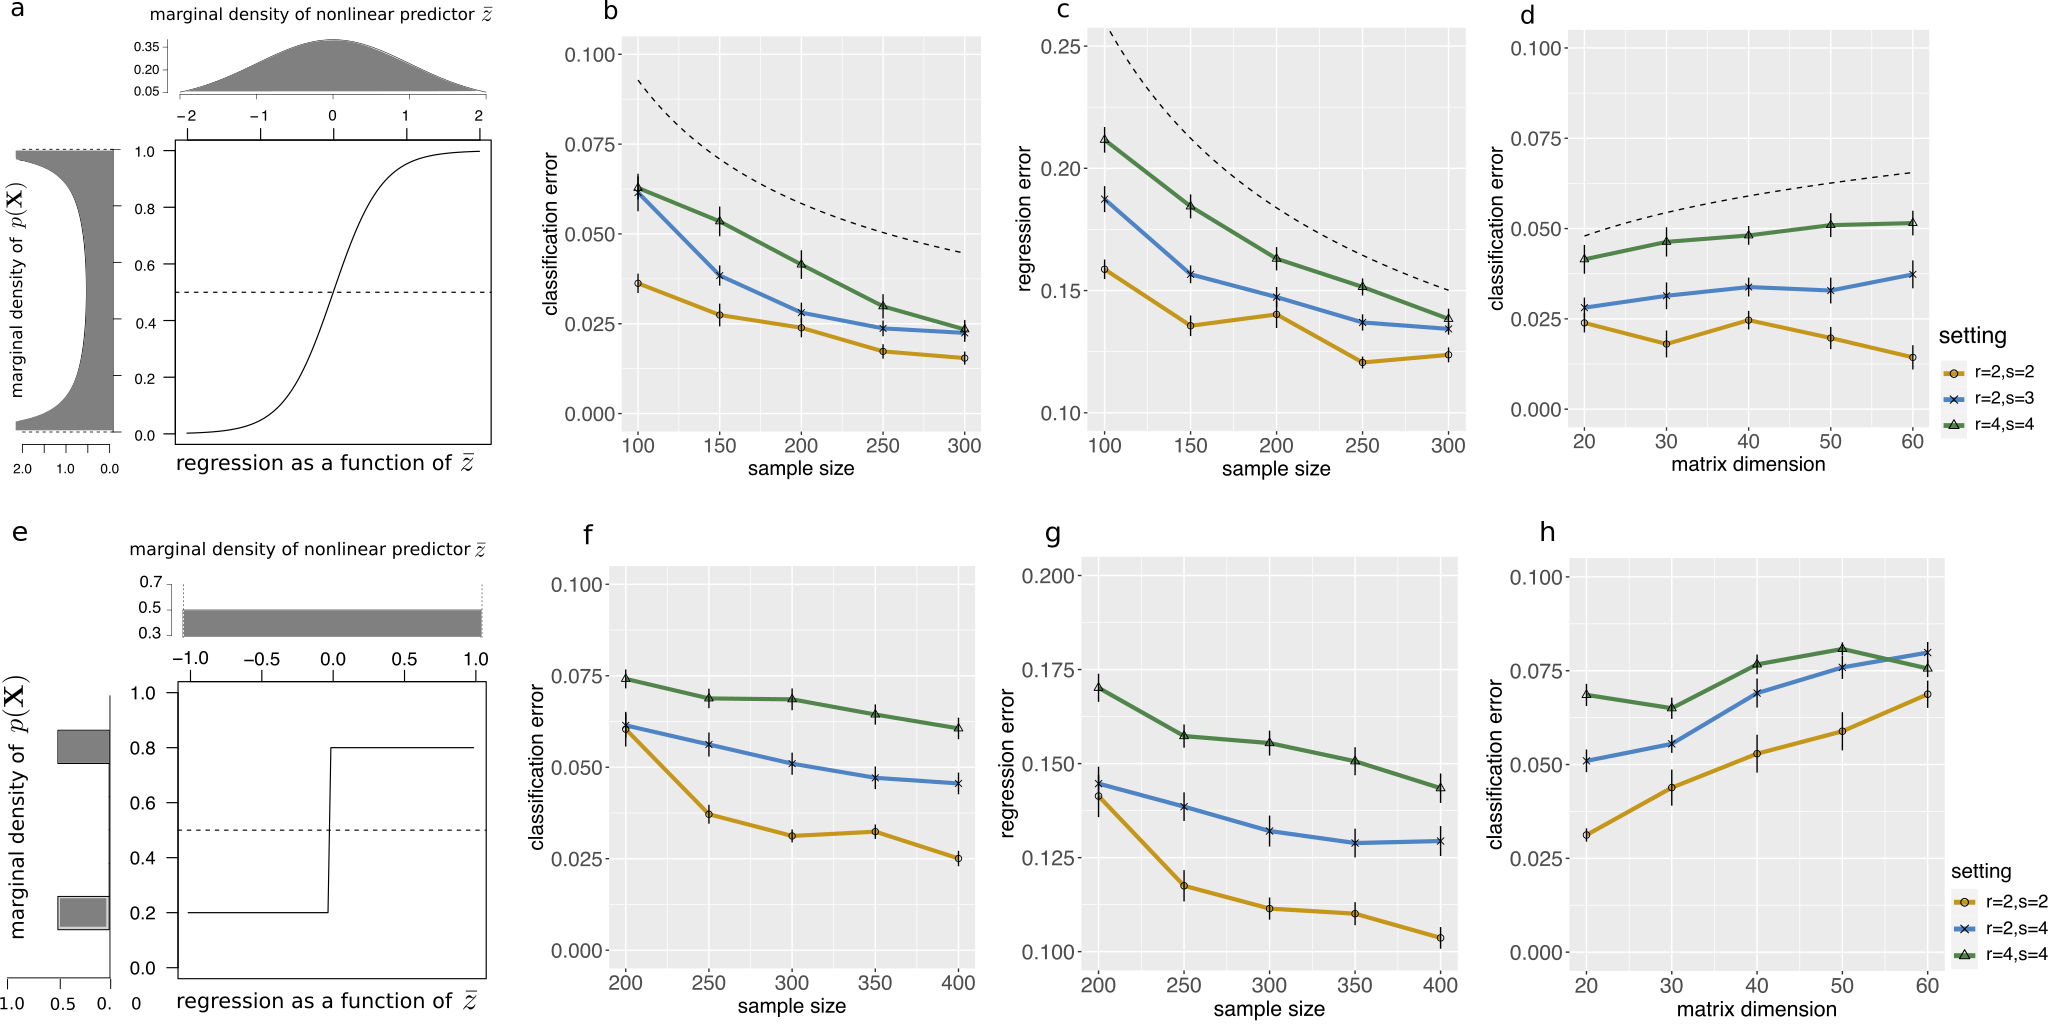
\includegraphics[width=\textwidth]{combined.pdf}
    \caption{Performance for matrix classification and regression. (a) Relationship between the nonlinear predictor $\bar z$ and the Bernoulli probability $p(\mX)$. The distribution for each is plotted on the top and left side, respectively. (b) classification error with sample size. (c) classification error with matrix dimension. (d) regression error with sample size. The dash line in panels (b)-(d) represent theoretical rates $\tO(n^{-2/3})$, $\tO(\log d)$, and $\tO(n^{-1/2})$, respectively.}\label{fig:logistic}
\end{figure}

The second experiment evaluates the impact of matrix dimension to classification accuracy. We fix the sample size $n=200$ and let the matrix dimension $d$ increase. Figure~\ref{fig:logistic}c plots the classification error versus the dimension $d$. We find that the error increases slowly and is well controlled by the log rate.  The ability to effectively control massive noisy features highlights the benefit of our method in high dimensions. 

The third experiment investigates the task of matrix regression. We set the smoothing parameter $H=20$ and aggregated the multiple level-sets as in our proposal~\eqref{eq:large-margin}. Figure~\ref{fig:logistic}d shows the regression error measured by $L$-1 risk, evaluated on test data. Again, we find that the regression error decays polynomially in sample size. Note that our matrix-valued feature has ambient dimension $30\times 30=900$ whereas the sample size is on the order of hundreds. Nevertheless, our nonparametric method consistently learns the function $p$ from limited data without a priori functional form.


 


\subsection{Comparison with other methods}\label{sec:comparison}
Next, we compare our Nonparametric matrix regression ({\bf \small NonparaM}) with several popular alternative methods: Unstructured regular lasso ({\bf \small Lasso},~\cite{friedman2010regularization}), Parametric regression for network predictors with group lasso ({\bf \small LogisticM},~\cite{relion2019network}), and Convolutional Neural Network ({\bf \small CNN}) with two hidden layers implemented in Keras \citep{chollet2015keras}. We choose a range of representative methods and aims to investigate the benefit of each approach. The \Lasso serves as a baseline to assess the gain of matrix-valued predictors over vector-valued predictors. 
Among the three methods that allow matrix-valued inputs, \CNN and \NonparaM provide nonparametric approaches and \LogisticM provide a parametric approach. 

\begin{figure}[ht]
    \centering
    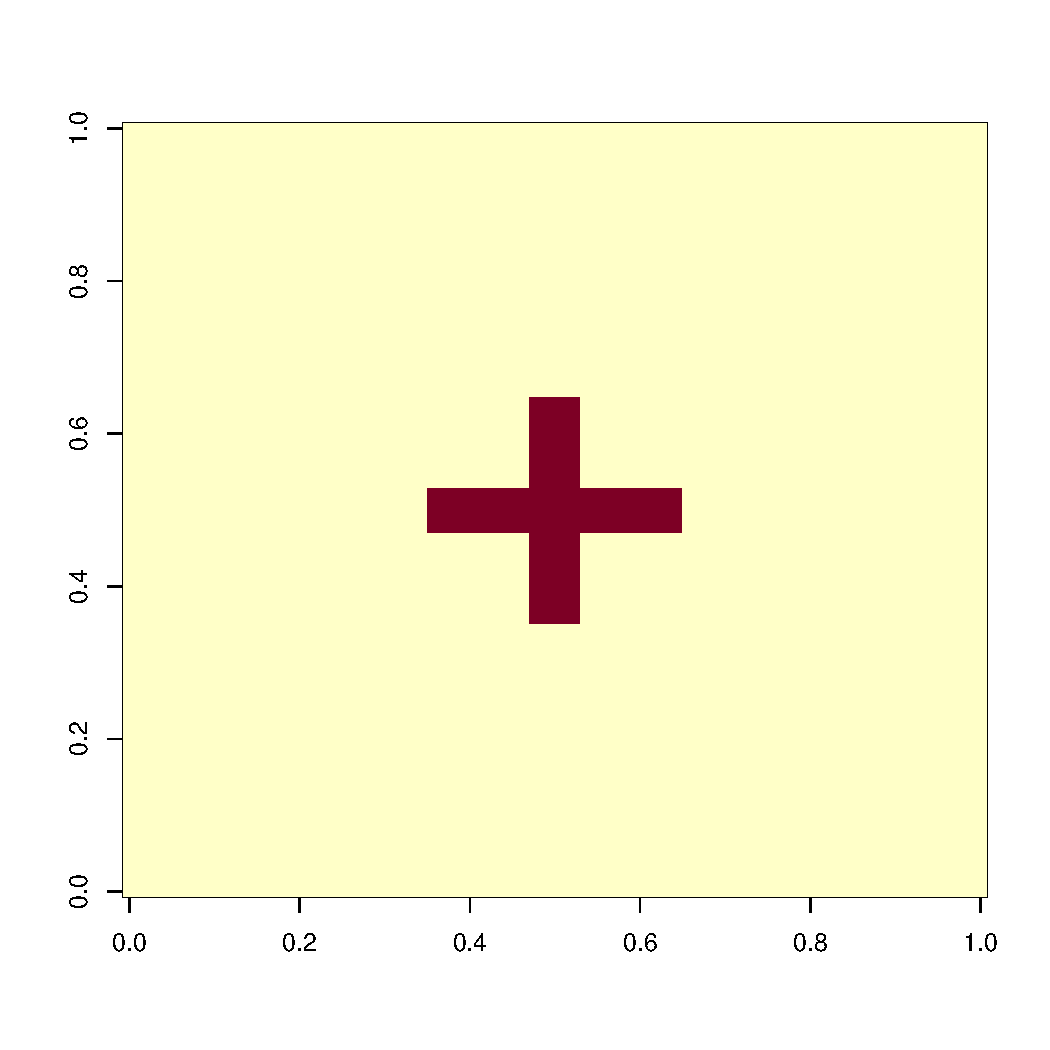
\includegraphics[width=4cm]{cross.pdf}
      \includegraphics[width=4cm]{block.pdf}
        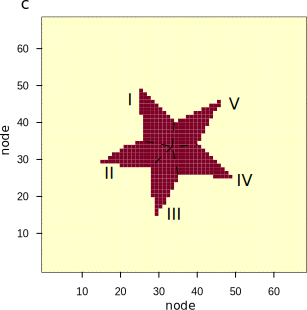
\includegraphics[width=4cm]{star.pdf}
          \includegraphics[width=4cm]{circle.pdf}
            
          \caption{Rank of support matrices: 3 (cross), 7 (block), almost full-rank (star), almost full-rank (circle)}\label{fig:region}
\end{figure}

For fair comparison, we adopt similar simulation setup as in~\cite{relion2019network}, expecting that we add more challenging network patterns in order to assess model misspecification. We draw a sample of $\pi$'s i.i.d.\ from Uniform[0,1], and simulate $y|\pi\sim \text{Ber}(\pi)$. Given $\pi\in[0,1]$, the network predictor is simulated from $\mX|\pi = (\pi-1/2)^2\mB_\pi+\mB_0 + \mE$, where $\mB_0$ is a baseline matrix, $\mB_\pi\in\{0,1\}^{d\times d}$ indicates the active regions of connectivity among $d$ nodes, and $\mE$ is the noise matrix consisting of i.i.d.\ N(0,\ 0.01) entries. The support of the matrix $\mB_\pi$ varies depending on the range in which $\pi\in[0,1]$ falls. We divide the range $[0,1]$ into several equally spaced intervals, e.g., $[0,1/4],\ldots,[3/4,1]$. Figure~\ref{fig:region} illustrates the four patterns of $(\mB_\pi)_{\pi\in[0,1]}$. We refer to the four patterns as ``cross'', ``block'', ``star'', and ``circle''. The baseline $\mB_0$ is set to be a matrix with entry 1 in the depicted region and zero otherwise. We set $d=68$, a training  size $n=160$, and a test size $80$. 





% In the noiseless case, the cross and block patterns are low-rank ($r = 3$ and 5, respectively), whereas the star and circle patterns are nearly full-rank (numerical rank $r\approx 30$ on the supported submatrix). In our simulation with noisy observation, we select the rank and sparsity parameters $(r,s)$ by 5-fold cross validation within training data. The hyperparameters for the other three methods are selected by either default setting ({\bf \small LogisticM}) or cross validation ({\bf \small Lasso}, {\small \bf CNN}). 

\begin{figure}[ht]
    \centering
    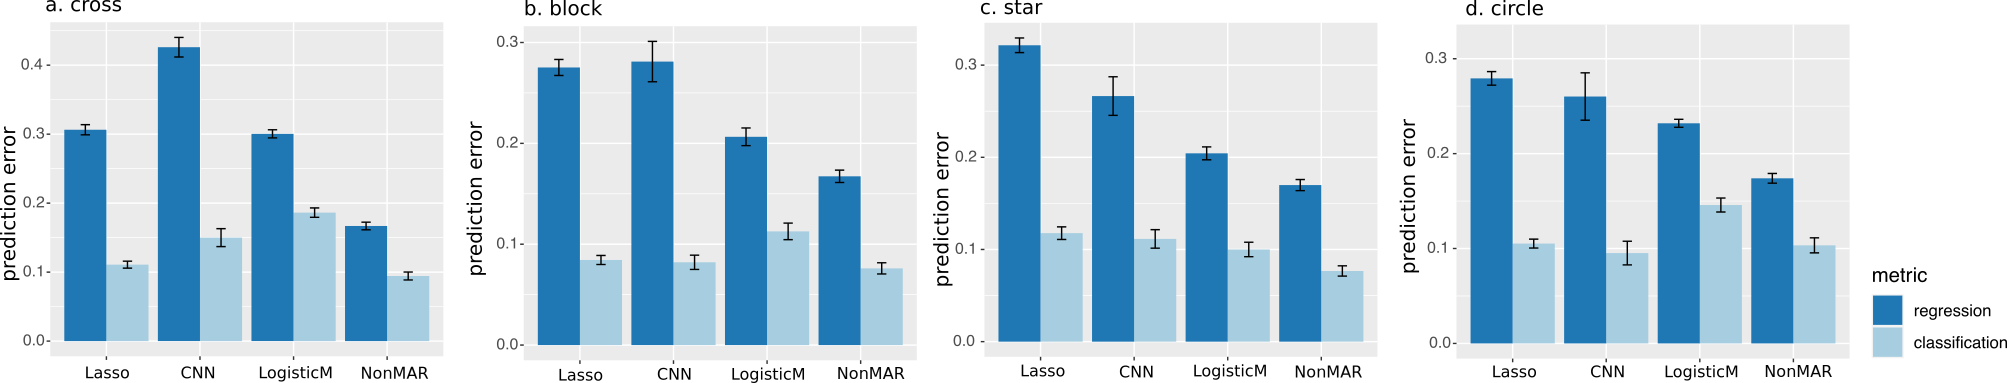
\includegraphics[width=\textwidth]{error_tot_comb2.pdf}
    \caption{Comparison of prediction errors between various methods. (a)-(d) represent four different activation patterns. }\label{fig:compare}
\end{figure}

Figure~\ref{fig:compare} compares the out-of-sample prediction between different methods. For regression problem, we find that \NonparaM consistently outperforms others, and the reduction in error is substantial. For example, the relative reduction using \NonparaM over the next best approach, {\bf \small LogisticM}, is over 20\% for models 1 and 4, and over 15\% for models 2 and 3. The results show the benefit of our nonparametric approache by allowing more flexible functional space. Furthermore, we find that neither \Lasso nor \CNN has satisfactory regression performance. One possible reason is that these two methods fail to appropriately incorporate the network structure of the predictors. The \Lasso takes vectorized matrices as inputs and therefore losses the two-way pairing information. On the other hand, \CNN assumes spacial ordering within the $d=64$ row/column indices. Although local similarity is an appropriate model for imaging, the indexing of rows/columns are meaningless for networks. Methods that are index-invariant (\LogisticM and {\bf \small NonparaM}) show better performance.  The results demonstrate the advantages of our nonparametric approach on the task of network regression. 



We also report the accuracy on classification which is an intermediate step of regression. Figure~\ref{fig:compare} shows the favorable performance of our method especially when compared to {\bf \small LogisticM}. Among the four models of active regions, our method performs the best in all three. The only exception is the circle model where the \CNN has a lower error by a slight margin. This is perhaps due to the fact that circle pattern is nearly full rank which favors complicated models such as {\bf \small CNN}. Nevertheless, our method \NonparaM achieves stable performance in spite of its simplicity. 


% \begin{table}[ht]
% \centering
% \begin{tabular}{ccccc}
% Method& Cross Pattern & Block Pattern &Star Pattern & Circle Pattern\\
% \hline
% Lasso&.51(.003)&.52(.003)&.51(.005)&.51(.002)\\
% %LogisticM&.89(.04)&.96(.04)&.93(.04)&.94(.03)\\
% NonparaM&.87(.03)&.93(.04)&.84(.03)&.82(.03)\\
% \end{tabular}
% \caption{comparison for active region selection under different pattern models. }\label{tab:selection}
% \end{table}
\begin{figure}[ht]
    \centering
   \includegraphics[width=4cm]{est_cross.pdf}
          \includegraphics[width=4cm]{est_block.pdf}
        \includegraphics[width=4cm]{est_star.pdf}
          \includegraphics[width=4cm]{est_circle.pdf}
 \caption{Rank of support matrices: 3 (cross), 7 (block), almost full-rank (star), almost full-rank (circle)}\label{fig:compare2}
\end{figure}


 Figure~\ref{fig:compare2} shows the example results returned by {\bf \small NonparaM}.  The results demonstrate that our \NonparaM enjoys the accurate prediction as a nonparametric approach, while inheriting the interpretability of parametric approaches. 


\vspace{-.5cm}
\section{Conclusion}
\vspace{-.3cm}
We have developed the learning framework for the relationship between a binary label response and a high-ddimensional matrix-valued predictor. Our method respects the matrix structure of the predictors and produces interpretable result with nonparametric approach. Both theoretical and numerical results are provided to demonstrate the comepetetive performance of our estimation. The work unlocks several directions of future research. Extension to multilclass probability estimation and to nonlinear boundaries through kernel methods would be of interest. Application to nonparametic way for matrix completion and denoising problem warrants future research.

\singlespacing
\bibliographystyle{chicago}
\bibliography{tensor_wang}



\end{document}



